\documentclass{beamer}

\usepackage{relsize}
\usepackage{color}

\begin{document}

\begin{frame}
\frametitle{Intervenants}
\begin{itemize}
\item \textbf{Beno\^{i}t Valiron} (responsable du cours - \textcolor{blue}{ benoit.valiron@centralesupelec.fr} - remplac\'{e} par BM)\\~\\
\item \textbf{Bertrand Marchand} (\textcolor{blue}{bertrand.marchand@lix.polytechnique.fr} - TP 1)\\~\\
\item \textbf{Simon Martiel} (\textcolor{blue}{simon.martiel@atos.net} - TP 2)
\end{itemize}
\end{frame}

\begin{frame}
\frametitle{Usual gates}
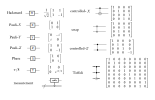
\includegraphics[width=\textwidth]{quantum_gates.pdf}
\end{frame}

\begin{frame}
\frametitle{Example of a quantum circuit: QFT}

\begin{center}
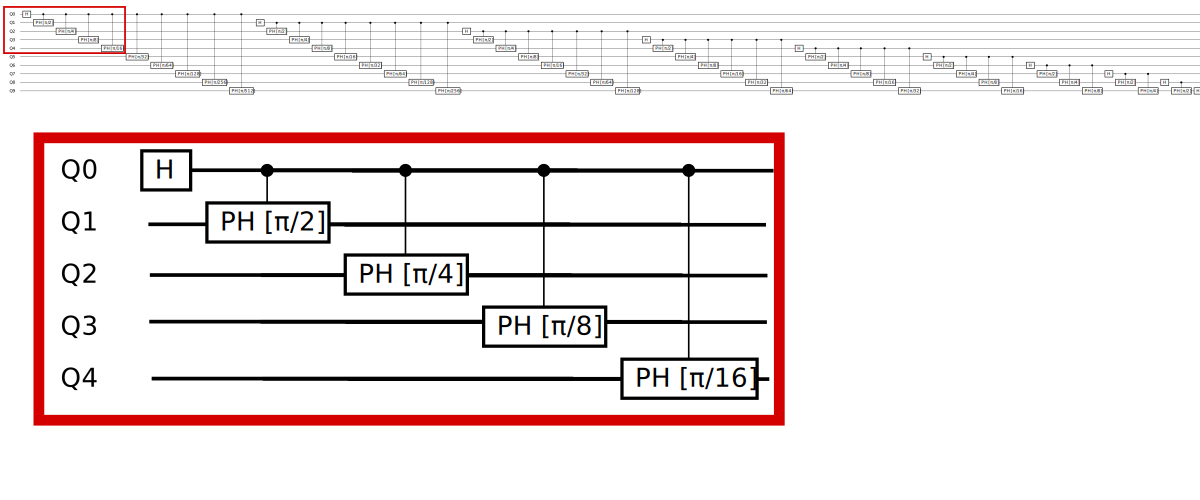
\includegraphics[width=\textwidth]{qft.pdf}
\end{center}

\end{frame}

\begin{frame}
\frametitle{Oracle for SHA256}

\begin{center}
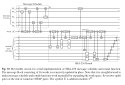
\includegraphics[width=.9\textwidth]{sha256.pdf}
\end{center}
\relsize{-1}
{
from \emph{Time–space complexity of quantum search algorithms in symmetric cryptanalysis: applying to AES and SHA-2}, Kim et al., 2018.
}

\end{frame}

\begin{frame}
\frametitle{Overview of quantum algorithms}

\begin{itemize}
\item \textbf{Quantum search algorithms} Use $O(\sqrt{N})$ calls to an oracle $O_f$ to identify
elements with $f(x)=1$ in a list of $N$ elements.\\
 $\quad\rightarrow$ generalizations: \textbf{quantum walks}
\item \textbf{QFT-based algorithms}
\begin{itemize}
\item \textbf{Shor's algorithm } to factor integers and other \textbf{order-finding algorithms}
\item \textbf{Quantum chemistry} (and the solving of other Physics/Chemistry problems) through phase estimation.
\item \textbf{Quantum linear algebra} and machine learning or other applications.
\end{itemize}                    
\end{itemize}

\end{frame}

\end{document}
